\documentclass[conference]{IEEEtran}

\usepackage{color}
\usepackage{mathtools}
\usepackage{fullpage}
\usepackage{algorithmic}
\DeclareMathOperator*{\argmin}{argmin}
\algsetup{linenosize=\small}
\usepackage[table,xcdraw]{xcolor}
\usepackage{multirow}
\usepackage[super]{nth}
\usepackage{graphicx}
\usepackage{caption}
\usepackage{subcaption}
\usepackage{setspace}
\usepackage{textcomp}
\usepackage{xspace}
\usepackage{siunitx}
\usepackage{epsfig}
\usepackage{epstopdf}
\usepackage{soul}
\usepackage{url}
\usepackage{tablefootnote}
\DeclareMathOperator{\E}{\mathbb{E}} % Expectation Symbol
\usepackage{graphicx}
\usepackage[labelformat=simple]{subcaption}
\usepackage{epsfig} % To display images
\usepackage{amsmath,amssymb}
\usepackage[linesnumbered,ruled]{algorithm2e}
\usepackage{makecell}
\usepackage{multirow}
\usepackage{booktabs}
\usepackage{adjustbox}
\usepackage[space]{cite}
% correct bad hyphenation here
\hyphenation{}

\usepackage[labelformat=simple]{subcaption}
\renewcommand\thesubfigure{(\alph{subfigure})}
\usepackage[font=scriptsize]{subcaption}

%\setlength{\belowcaptionskip}{-1pt}

\begin{document}
	
	%
	% paper title
	% Titles are generally capitalized except for words such as a, an, and, as,
	% at, but, by, for, in, nor, of, on, or, the, to and up, which are usually
	% not capitalized unless they are the first or last word of the title.
	% Linebreaks \\ can be used within to get better formatting as desired.
	% Do not put math or special symbols in the title.
	\title{Implications of Decentralized Q-Learning Resource Allocation in Wireless Networks}
	
	% author names and affiliations
	% use a multiple column layout for up to three different
	% affiliations
	\author{
		\IEEEauthorblockN{Francesc Wilhelmi, Boris Bellalta}
		\IEEEauthorblockA{
			Wireless Networking (WN-UPF)\\
			Univ. Pompeu Fabra\\
			Barcelona}
		\and
		\IEEEauthorblockN{Cristina Cano}
		\IEEEauthorblockA{WINE Group\\ Univ. Oberta de Catalunya\\
		Castelldefels, Barcelona}
		
		\and
		\IEEEauthorblockN{Anders Jonsson}
		\IEEEauthorblockA{
			Art. Int. and Mach. Learn. (AIML-UPF)\\
			Univ. Pompeu Fabra\\
			Barcelona}
	}
	
	% make the title area
	\maketitle
	
	% As a general rule, do not put math, special symbols or citations
	% in the abstract
	\begin{abstract}
		%% Text of abstract
		Reinforcement Learning is gaining increasing attention by the wireless networking community due to its potential to learn good-performing configurations only from the observed results. In this work we propose a Stateless variation of Q-learning, which is applied to exploit spatial reuse in a wireless network. In particular, we allow nodes to modify both their transmission power and channel solely based on the experienced throughput. We concentrate in a completely decentralized scenario in which no information about neighbouring nodes is available to the learners. Our results show that although the algorithm is able to find the best-performing actions to enhance aggregate throughput, there is high variability in the throughput experienced by the individual networks. We identify the cause of this variability to be the adversarial setting of our setup in which the set of most played actions provide intermittent good/poor performance depending on the neighbouring decisions. The effect of the algorithm's learning parameters on this variability is also studied.
		
	\end{abstract}
	
	% For peer review papers, you can put extra information on the cover
	% page as needed:
	% \ifCLASSOPTIONpeerreview
	% \begin{center} \bfseries EDICS Category: 3-BBND \end{center}
	% \fi
	%
	% For peerreview papers, this IEEEtran command inserts a page break and
	% creates the second title. It will be ignored for other modes.
	\IEEEpeerreviewmaketitle
	
	%%%%%%%%%%%%%%%%%%%%%%%%%%%%%%%%%%%%%%%%%%%%%%%%
	%%%%%%  I. INTRODUCTION %%%%%%
	%%%%%%%%%%%%%%%%%%%%%%%%%%%%%%%%%%%%%%%%%%%%%%%%
	\section{Introduction}
	% no \IEEEPARstart	
	Reinforcement Learning (RL) has recently spread use in the wireless communications field to solve many kind of problems such as Access Point (AP) association, channel selection or transmit power adjustment \cite{nie1999qlearning, maghsudi2015joint}, as it allows learning good-performing configurations only from the observed results. Among these, Q-learning has been applied to dynamic channel assignment in mobile networks in \cite{nie1999qlearning} and to automatic channel selection in Femto Cell networks in \cite{bennis2010q}. However, the case of a fully decentralized scenario has not yet been considered.  
	
	In this work we propose a stateless variation of Q-learning in which nodes select the transmission power and channel to use solely based on the resulting throughput. We concentrate on a fully decentralized scenario where no information about the other nodes actions and resulting performance is available to the learners. Note that inferring the throughput of neighbouring nodes allocated to different channels is costly as periodic sensing in the other channels would then be needed. We aim to characterize the performance of Q-learning in such scenarios, obtaining insight on the most played actions (i.e., configurations selected) and the resulting performance. We observe that when no information about the neighbours is available to the learners, these will tend to apply selfish strategies that result in alternating good/poor performance depending on the actions of the others. In such scenarios, we show that the use of Q-learning allows each network to find the best-performing actions, though without reaching a steady solution. Note that achieving a steady solution in a decentralized environment relies in finding a Nash Equilibrium, a concept used in Game Theory to define a set of individual strategies that maximize the profits of each player in a non-cooperative game, regardless of the others' strategy. Formally, a set of best player actions $a^* = (a_1^*, ..., a_n^*) \in A$ leads to a Nash Equilibrium if $a_i^* \in B_i(a_{-i}^*), \forall i \in N$, where $B_i(a_{-i})$ is the best response to the others actions ($a_{-i}$). Thus, the consequences of not reaching a Nash Equilibrium can have an impact on performance variability.
	
	In addition, we look at the resulting performance when varying several parameters intrinsic to the learning algorithm, which results to be helpful to understand the interactions among the degree of exploration and the variability of the resulting performance. 
	
	The remaining of this document is structured as follows: in Section \ref{section:qlearning} our Stateless variation of Q-learning and its practical implementation for the resource allocation problem in WNs is presented. Then, in Section \ref{section:system_model} we present the simulation scenario and considerations. Simulation results are later discussed in Section \ref{section:performance_evaluation}. Finally, some final remarks are provided in Section \ref{section:conclusions}. 
	
	%%%%%%%%%%%%%%%%%%%%%%%%%%%%%%%%%%%%%%%%%%%%%%%%
	%%%%%%  II. DECENTRALIZED LEARNING ALGORITHMS %%%%%%
	%%%%%%%%%%%%%%%%%%%%%%%%%%%%%%%%%%%%%%%%%%%%%%%%
	\section{Decentralized Stateless Q-learning for enhancing Spatial Reuse in a WN}
	\label{section:qlearning}	
	Q-learning \cite{sutton1998reinforcement, watkins1992q} is an RL technique that enables an agent to learn the optimal policy to follow in a given environment. A set of possible states (that describe the status of the environment) and actions are defined. In particular, an agent maintains an estimate of the expected long-term discounted reward for each state-action pair, and selects actions with the aim of maximizing it. The expected cumulative reward $\text{V}^\pi(s)$ is given by:
	\begin{equation}
	\label{eq:ql_reward_policy}
	\text{V}^\pi(s) = \lim_{N \rightarrow \infty} \mathop{\mathbb{E}}\Big(\sum_{t=1}^{N} r_t^\pi(s)\Big),
	\nonumber
	\end{equation}
	where $r_t^\pi(s)$ is the reward obtained at iteration $t$ after starting from state $s$ and by following policy $\pi$. Since the reward may easily get unbounded, a discount factor parameter ($\gamma < 1$) is used. The optimal policy $\pi^*$ that maximizes the total expected reward is obtained by using the Bellman's Optimality Equation \cite{sutton1998reinforcement}:	
	\begin{equation}
	Q^*(s,a) = \mathbb{E} \Big\{r_{t+1} + \gamma \text{max}_{a'} Q^*(s_{t+1},a') | s_t = s, a_t = a\Big\}. \nonumber
	\end{equation}	
	Henceforth, Q-learning receives information about the current state-action tuple $(s_t,a_t)$, the generated reward $r_t$ and the next state $s_{t+1}$, in order to update the Q-table $\hat{Q}(s_t,a_t)$: 	
	\begin{equation}
	\hat{Q}(s_t,a_t)\leftarrow (1-\alpha_t) \hat{Q}(s_t,a_t) + \alpha_t (r_t + \gamma (\underset{a'}{\text{max}}\hat{Q}(s_{t+1},a')),
	\nonumber
	\end{equation}	
	where $\alpha_t$ is the learning rate at time $t$, and $\underset{a'}{\text{max}}\hat{Q}(s_{t+1},a')$ is the best estimated value for the next state $s_{t+1}$. The optimal solution is achieved with probability 1 if $\sum_{t=0}^{\infty} \alpha_t = \infty$, and $\sum_{t=0}^{\infty} \alpha_t^2 < \infty$, which satisfies that $\underset{t \rightarrow \infty}{\lim} \hat{Q}(s,a) = Q^*(s,a)$.
	Since we focus on a completely decentralized scenario where no information about the other nodes is available, the system can then be fully described by the set of actions and rewards.\footnote{We note that local information such as the observed instantaneous channel quality could be incorporated in the state definition. However, such a description of the system entails increased complexity.} Thus, we apply a Stateless variation of the original Q-learning algorithm. We then consider each WN to be an agent implementing Q-learning through an $\varepsilon$-greedy action-selection strategy, so that actions $a \in \mathcal{A}$ correspond to all the possible configurations that can be chosen with respect to the channel and transmit power. The implementation details are described in Algorithm \ref{alg:qlearning}.
		
	\begin{algorithm}
		\SetKwInOut{Input}{Input}
		\SetKwInOut{Output}{Output}		
		Function Stateless Q-learning $(\text{SINR},\mathcal{A})$\;
		\Input{SINR: Signal-to-Interference-plus-Noise Ratio sensed at the STA\\$\mathcal{A}$: set of possible actions in \{1, ..., K\}}
		\Output{$\overline{\Gamma}$: Mean throughput experienced in the WN}
		initialize: $t=0$, $\hat{Q}(a_i) = 0, \forall a_i \in \mathcal{A}$\\
		\While{active}
		{
			Select $a_i$  $\begin{cases}
			\underset{i=1,...,K}{\text{argmax }} \hat{Q}(a_i), & \text{with prob } 1 - \varepsilon\\
			i \sim \mathcal{U}(1, K),, & \text{otherwise}
			\end{cases}$\\
			Observe reward $r_{a_i} = \frac{\Gamma_{a_i}}{\Gamma^*}$ \\
			$\hat{Q}(a_i) \leftarrow \hat{Q}(a_i) + \alpha \cdot (r_{a_i} + \gamma \cdot \max(\hat{Q}(:)) - \hat{Q}(a_i))$\\
			$\varepsilon_t \leftarrow \varepsilon_0 / \sqrt{t}$ \\	
			$ t \leftarrow t + 1$
		}
		\caption{Stateless Q-learning}
		\label{alg:qlearning}
	\end{algorithm}
	
	%%%%%%%%%%%%%%%%%%%%%%%%%%%%%%%%%%%%%%%%%%%%%%%
	%%% III. SYSTEM MODEL %%%
	%%%%%%%%%%%%%%%%%%%%%%%%%%%%%%%%%%%%%%%%%%%%%%%
	\section{System model}
	\label{section:system_model}	
	We consider a scenario at which several WNs are placed in a 3D-map (with parameters described later in Section \ref{section:simulation_parameters}), each one formed by an Access Point (AP) transmitting to a single Station (STA). 
	
	%------------------------
	% Channel modelling
	%------------------------
	\subsection{Channel modelling}
	\label{section:channel_modelling}
	
	Path-loss and shadowing are modelled by the following log-distance model:	
	\begin{align}
	\text{PL}_{i,j} = \text{P}_{{\rm tx}_i} - \text{P}_{{\rm rx}_j} & = \nonumber \\ = \text{PL}_0 + & 10 \cdot \alpha \cdot \log_{10}(d_{i,j}) + \text{G}_{{\rm s}} + \frac{d_{i,j}}{d_{{\rm obs}}} \text{G}_{{\rm o}}, \nonumber
	\end{align}
	where $\text{P}_{{\rm tx}_i}$ is the transmitted power in dBm by WN $w_i$, $\text{P}_{{\rm rx}_j}$ is the power in dBm received at WN $w_j$, $\text{PL}_0$ is the path-loss at $1$ m in dB, $d$ is the distance between the transmitter and the receiver in meters, $\text{G}_{{\rm s}}$ is the shadowing loss in dB, and $\text{G}_{{\rm o}}$ is the obstacles loss in dB. Note that we also include the factor $d_{{\rm obs}}$, which represents the distance between two obstacles in meters. 
	
	%------------------------
	% Throughput calculation
	%------------------------
	\subsection{Throughput calculation}
	\label{section:throughput_calculation}
	
	By using the power received and the interference, we calculate the resulting throughput of each WN $w_i$ by using the Shannon Capacity.
	\begin{equation}
	\Gamma_{i,t} = B \cdot \log_{2}(1 + \text{SINR}_{\text{w}_i, t}),
	\nonumber
	\label{eq:shannon_capacity}
	\end{equation}
	where $B$ is the channel width and the experienced SINR is given by:
	\begin{equation}
	\text{SINR}_{{\text{w}_i},t} = \frac{\text{P}_{{\text{w}_i},t}}{\text{I}_{{\text{w}_i},t}+\text{N}} \: [dB],
	\label{eq:sinr}
	\end{equation}
	where $\text{P}_{{w_i},t}$ and $\text{I}_{{w_i},t}$ are the received power and the sum of the interference at WN $w_i$ at time $t$, respectively, and N is the floor noise power. For each STA in a WN, the interference is considered to be the total power received from all the APs of the other coexisting WNs $w_{j \neq i} \in \mathcal{W} $ as if they were continuously transmitting. Note that, adjacent channel interference is also considered in $\text{I}_{{w_i},t}$. We consider that the transmitted power leaked to adjacent channels is $20$ dBm lower for each channel separation.
	
	%------------------------
	% RL Considerations
	%------------------------
	\subsection{Reinforcement Learning Considerations}
	\label{section:rl_considerations}	
	During the learning process we assume that WNs select actions sequentially, so that at each learning iteration, every agent takes an action in an ordered way. The order at which WNs choose an action at each iteration is randomly selected at the beginning of it. The reward after choosing an action is set as:
	\begin{equation}
	R_{\text{w}_i,t} = {\frac{\Gamma_{\text{w}_i,t}}{{\Gamma_{\text{w}_i,t}^*}}},
	\label{eq:reward_generation}
	\nonumber
	\end{equation}
	where $\Gamma_{i,t}$ is the experienced throughput by $\text{w}_i$, and $\Gamma_{\text{w}_i, t}^* = B \cdot \log_{2}(1 + \text{SNR}_{\text{w}_i,t})$ is the maximum throughput at WN $w_i$ (i.e., when it uses the maximum transmission power and there is no interference).	
	
	%%%%%%%%%%%%%%%%%%%%%%%%%%%%%%%%%%%%%%%%%
	%%% IV. SIMULATION %%%
	%%%%%%%%%%%%%%%%%%%%%%%%%%%%%%%%%%%%%%%%%
	\section{Performance Evaluation}
	\label{section:performance_evaluation}	
	In this Section we introduce the simulation parameters and the considerations taken into account for the experiments.\footnote{The code used for simulations can be found at \url{https://github.com/wn-upf/Decentralized_Qlearning_Resource_Allocation_in_WNs.git}.}. Then, we show the main results.

	%------------------------
	% Simulation Parameters
	%------------------------
	\subsection{Simulation Parameters}
	\label{section:simulation_parameters}
	According to \cite{bellalta2016ax}, a typical high-density scenario for residential buildings contains $0.0033 \text{APs}/\text{m}^3$. We then consider a map scenario with dimensions $10\times5\times10$ m containing 4 WNs that form a grid topology in which STAs are placed at the maximum possible distance from the other networks. This toy scenario allows us to study the performance of Stateless Q-learning in a controlled environment. We consider that the number of channels is equal to half the number of coexisting WNs, so that we can study a challenging situation regarding the spatial reuse. Table \ref{tbl:simulation_parameters} details the parameters used.	
	\begin{table}[h!]
		\centering
		\resizebox{\columnwidth}{!}{%
			\begin{tabular}{|l|l|}
				\hline
				\textbf{Parameter}             & \textbf{Value}                      \\ \hline
				Map size (m)                    & $10\times5\times10$                  \\ \hline
				Number of coexistent WNs                    & 4  \\ \hline
				APs/STAs per WN                    & 1 / 1                                     \\ \hline
				Distance AP-STA (m)     & $\sqrt{2}$                         \\ \hline
				Number of Channels              & 2                               \\ \hline
				Channel Bandwidth (MHz)         & 20                                    \\ \hline
				Initial channel selection model & Uniformly distributed 
				\\ \hline
				TPC Values (dBm)                & \{5, 10, 15, 20\}                      \\ \hline				
				$\text{PL}_0$                   & 5
				\\ \hline
				$\text{G}_s$                   & Normally distributed with mean 9.5 
				\\ \hline
				$\text{G}_o$                  & Uniformly distributed with mean 30
				\\ \hline
				$f_w$  (meters to find a wall)                 & 5                        
				\\ \hline
				Noise level (dBm)               & -100                                  \\ \hline
				Traffic model                   & Full buffer (downlink)             \\ \hline           
			\end{tabular}
		}
		\caption{Simulation parameters}
		\label{tbl:simulation_parameters}
	\end{table}
	
	%------------------------
	% Optimality study
	%------------------------
	\subsection{Optimal solution}
	\label{section:optimal_solution}	
	We first identify the optimal solutions that maximize: $i$) the aggregate throughput,  and $ii$) the proportional fairness, which is computed as the logarithmic sum of the throughput experienced by each WN ($\sum_{\text{w}_i \in \mathcal{W}} \log(\Gamma_{\text{w}_i,t})$). 
	The optimal solutions are listed in Table \ref{tbl:optimal_configurations}. Note that, since the considered scenario is symmetric, there are two equivalent solutions. Note, as well, that in order to maximize the aggregate network throughput two of the WNs sacrifice themselves by choosing a lower transmit power. This result is then not likely to occur in an adversarial selfish setting.	
	\begin{table}[]
		\centering
		\resizebox{\columnwidth}{!}{%
			\begin{tabular}{|c|c|c|}
				\hline
				\textbf{WN id} & \textbf{\begin{tabular}[c]{@{}c@{}}Action that maximizes the \\ Aggregate Throughput\end{tabular}} & \textbf{\begin{tabular}[c]{@{}c@{}}Action that maximizes the\\ Proportional Fairness\end{tabular}} \\ \hline
				1 & 1 (2) & 7 (8) \\ \hline
				2 & 1 (2) & 8 (7) \\ \hline
				3 & 7 (8) & 7 (8) \\ \hline
				4 & 8 (7) & 8 (7) \\ \hline
			\end{tabular}	
		}		
		\caption{Optimal configurations (action indexes) to achieve the maximum network throughput and prop. fairness, resulting in 1124 Mbps and 891 Mbps, respectively. In parenthesis the analogous solution is shown. Actions indexes range from 1 to 8 and are mapped to (channel number, transmit power (dBm)): \{1,5\}, \{2,5\}, \{1,10\}, \{2,10\}, \{1,15\}, \{2,15\},\{1,20\} and \{2,20\}, respectively.}
		\label{tbl:optimal_configurations}
	\end{table}
	
	%------------------------
	% Tuning parameters
	%------------------------
	\subsection{Input Parameters Analysis}
	\label{section:practical_analysis}	
	We first analyse the effects of modifying $\alpha$ (the learning rate), $\gamma$ (the discount factor) and $\epsilon_0$ (the initial exploration coefficient of the $\epsilon$-greedy update rule) with respect to the achieved network throughput. We run simulations of $10000$ iterations and capture the results of the last $5000$ iterations to ensure that the initial transitory phase has ended. Each simulation is repeated $100$ times. 
	
	Figure \ref{fig:ql_alpha_gamma_epsilon_evaluation} shows the average aggregate throughput achieved for each of the proposed combinations. It can be observed that the best results with respect to the aggregate throughput, regarding both average and variance, are achieved when $\alpha = 1$, $\gamma = 0.95$ and $\varepsilon_0 = 1$. This means that for achieving the best results (i.e., high average aggregate throughput and low variance), the immediate reward of a given action must be considered rather than any previous information ($\alpha = 1$). We see that the difference between the pay-off offered by the best action and the current one must also be high ($\gamma = 0.95$). In addition, exploration must be highly boosted at the beginning ($\epsilon_0=1$). For this setting, the resulting throughput ($902.739$ Mbps) represents $80.29$\% of the one provided by the optimal configuration that maximizes the aggregate throughput (shown in Table \ref{tbl:optimal_configurations}). Regarding proportional fairness, the algorithm's resulting throughput is only $1.32$\% higher than the optimal (Table \ref{tbl:optimal_configurations}). 
	\begin{figure}[h!]
		\centering
		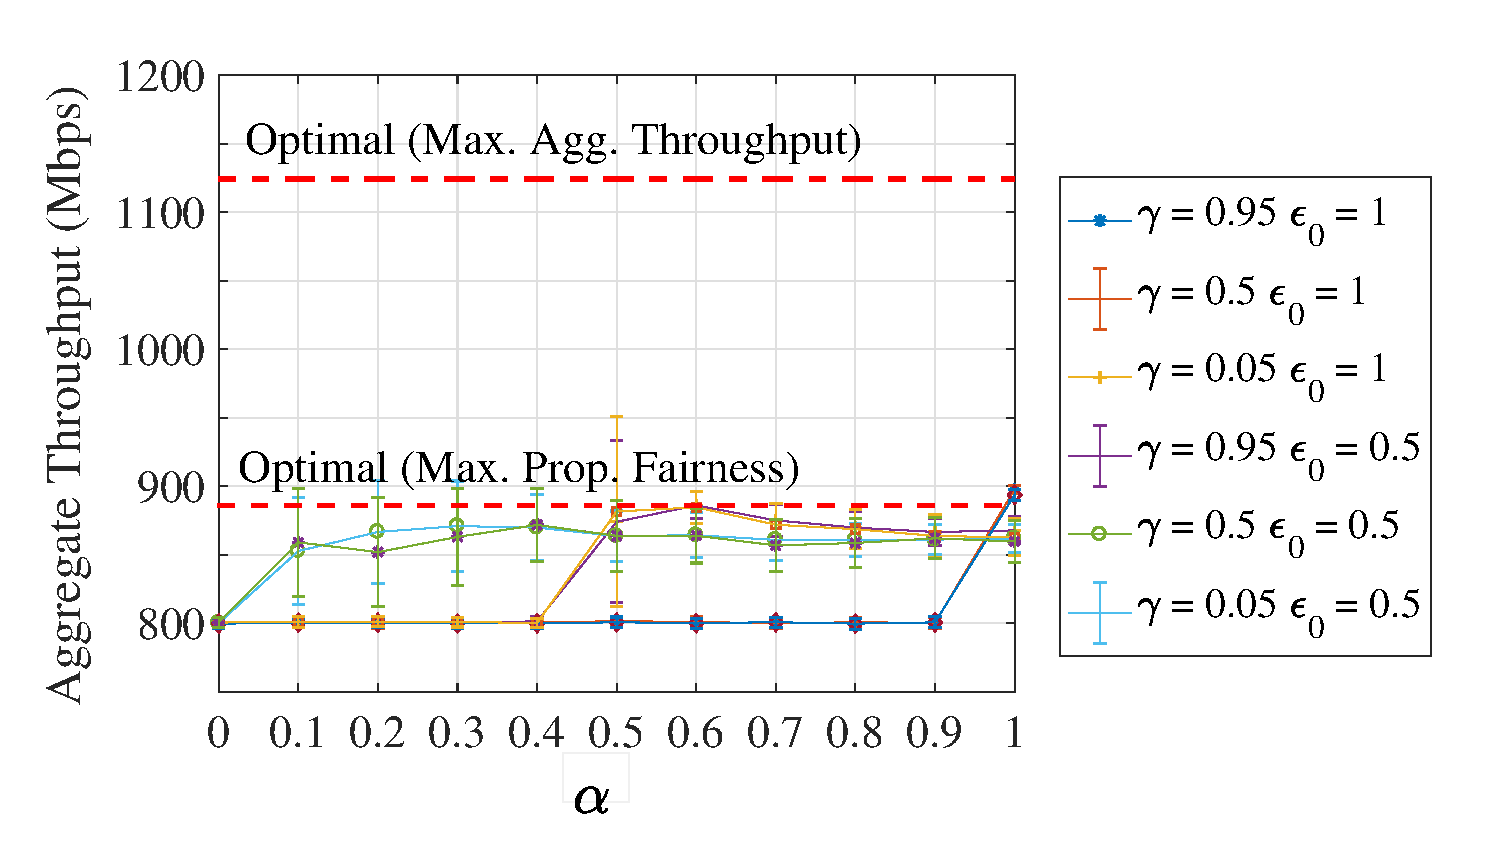
\epsfig{file=images/ql_tuning_params_fixed_map_last_5000_iterations.eps, width=8cm}
		\caption{Effect of $\alpha, \gamma$ and $\varepsilon_0$ in the average aggregate throughput ($100$ simulation runs per sample).}
		\label{fig:ql_alpha_gamma_epsilon_evaluation}
	\end{figure}	
	We also evaluate the relationship between different values of $\alpha$ and $\gamma$ in the average aggregate throughput and standard deviation (shown in Figure \ref{fig:ql_alpha_vs_gamma}).
	We can observe that we obtain consistently higher aggregate throughput when $\alpha > \gamma$. We also see that the variability between different simulation runs is much lower when the average throughput is higher. Additionally, we note a peak in the standard deviation when $\gamma \approx \alpha$ and $\gamma < \alpha$. 	
	\begin{figure}[t!]
		\centering
		\begin{subfigure}[(a)]{0.225\textwidth}
			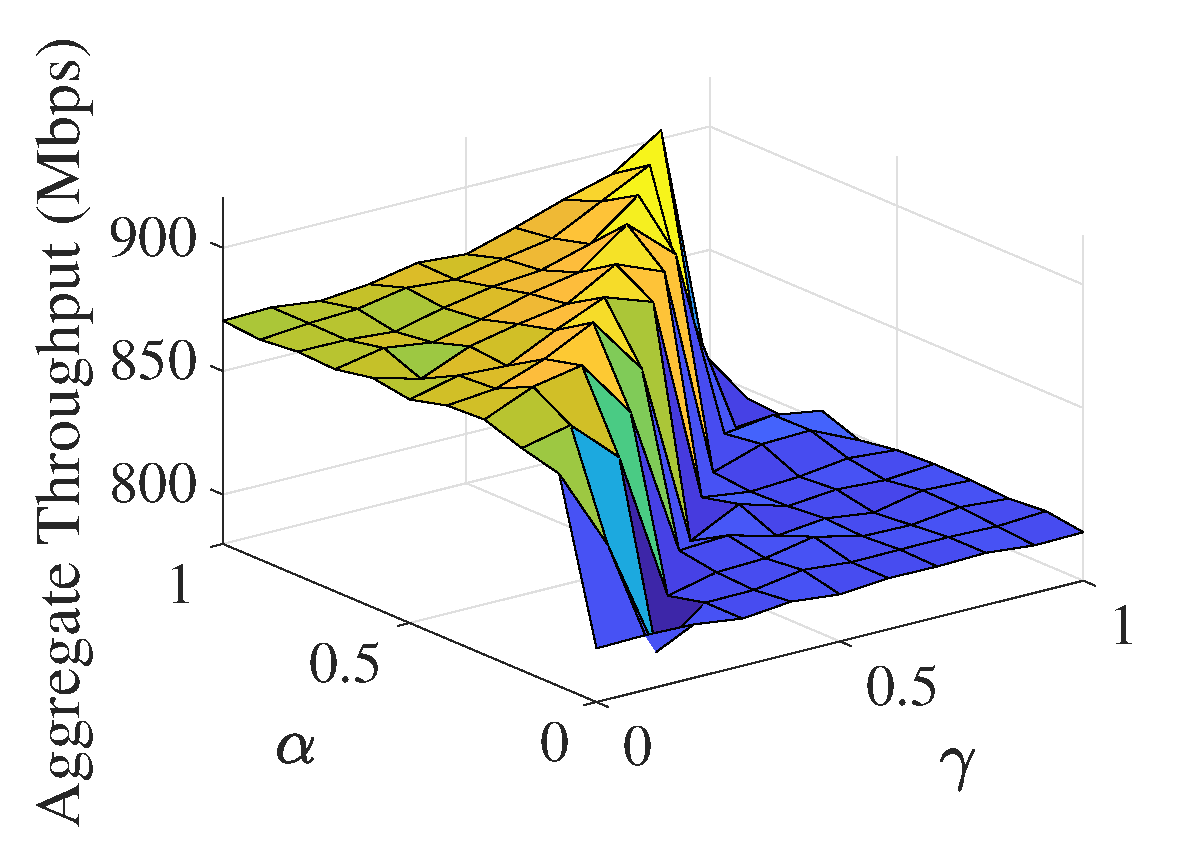
\includegraphics[width=\textwidth]{images/alpha_vs_gamma_avg_tpt_sqrt_epsilon}
			\caption{Av. aggregate throughput}
			\label{fig:alpha_vs_gamma_avg_tpt_sqrt_epsilon}
		\end{subfigure}
		\begin{subfigure}[(b)]{0.225\textwidth}
			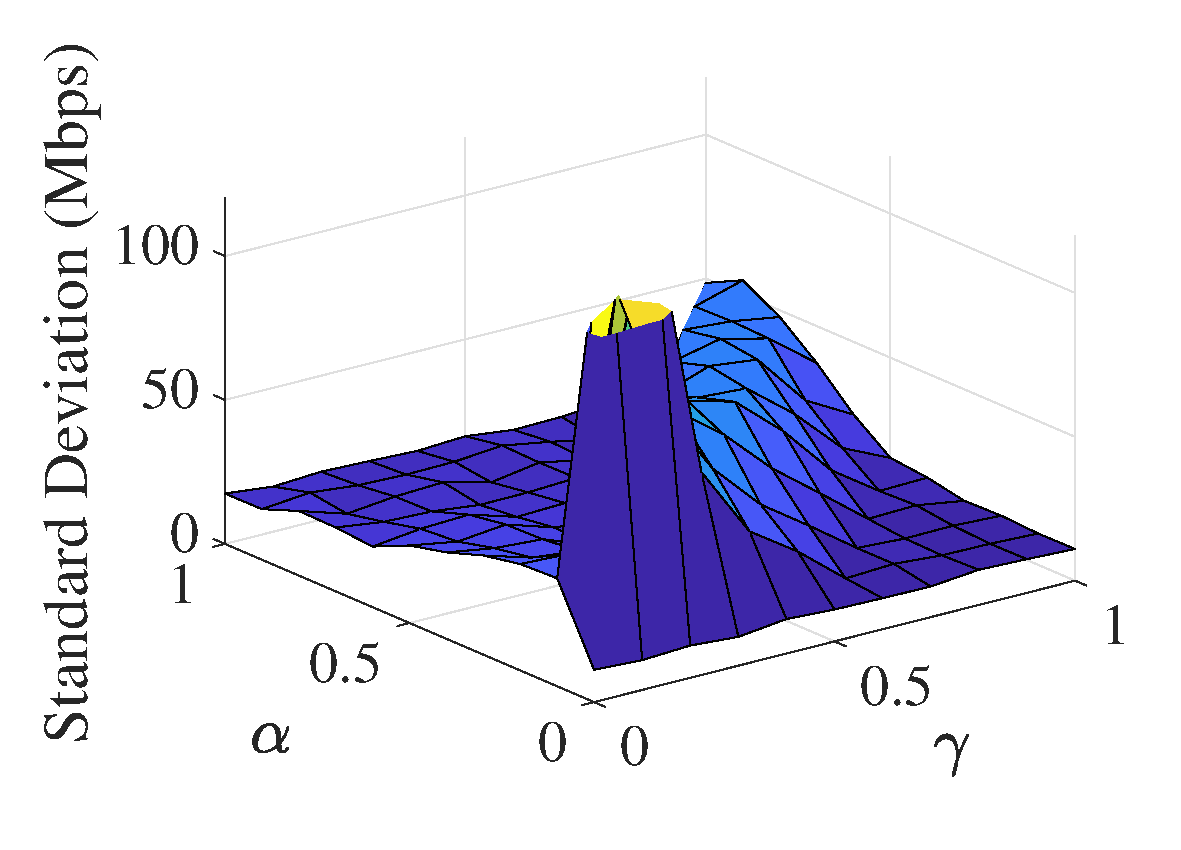
\includegraphics[width=\textwidth]{images/alpha_vs_gamma_std_sqrt_epsilon}
			\caption{Standard deviation}
			\label{fig:alpha_vs_gamma_std_sqrt_epsilon}
		\end{subfigure}
		\caption{Evaluation of $\alpha$ and $\gamma$.}
		\label{fig:ql_alpha_vs_gamma}
	\end{figure}
	To further understand the effects of modifying each of the aforementioned parameters, we show: $i$) the individual throughput experienced by each WN during the total $10000$ iterations of a single simulation run (Figure \ref{fig:ql_params_eval_individual_tpt}), $ii$) the average throughput experienced by each WN for the last 5000 iterations, also for a single simulation run (Figure \ref{fig:ql_params_eval_average_tpt}), and $iii$) the probability of choosing each action at each WN (Figure \ref{fig:ql_params_eval_actions_prob}). As it can be observed (Figures  \ref{fig:e_1_a1_g095}, \ref{fig:e_1_a_01_g_005}),
	%LAST-CC: digues a quines figures exactament tipus "(Figures XXa, XXb)"
	increasing the initial exploration coefficient ($\varepsilon_0$) allows for finding the best actions for each WN, so that the ones that provide consistently poor performance are discarded. However, the higher the exploration is, the higher the variability of the throughput experienced by each WN (Figures  \ref{fig:e_1_a1_g095_ind_tpt}, \ref{fig:e_1_a_01_g_005_ind_tpt}). By looking at the average throughput (Figure \ref{fig:ql_params_eval_average_tpt}), we see that a higher exploration allows for fairer distribution of the channel resources at the expense of suffering higher throughput variability. When comparing Figures \ref{fig:e_1_a1_g095} and \ref{fig:e_1_a_01_g_005}, we observe that for the former, there are two favourite actions that are being played the most, but for the latter there is only one preferred action. The lower the learning rate ($\alpha$), and consequently the discount factor ($\gamma$) due to the relationship shown in Figure \ref{fig:ql_alpha_vs_gamma}, the higher the probability of choosing a unique action, which results to be the one that provided the best performance in the past. The opposite occurs for higher $\alpha$ and $\gamma$ values, since giving more importance to the immediate reward allows for a reaction only to the recently-played actions of the neighbouring nodes: the algorithm is short-sighted. 
	
	%%% INDIVIDUAL THROUGHPUT FOR EACH PARAMETER	
	\begin{figure}[h!]
		\centering
		\begin{subfigure}[b]{0.225\textwidth}
			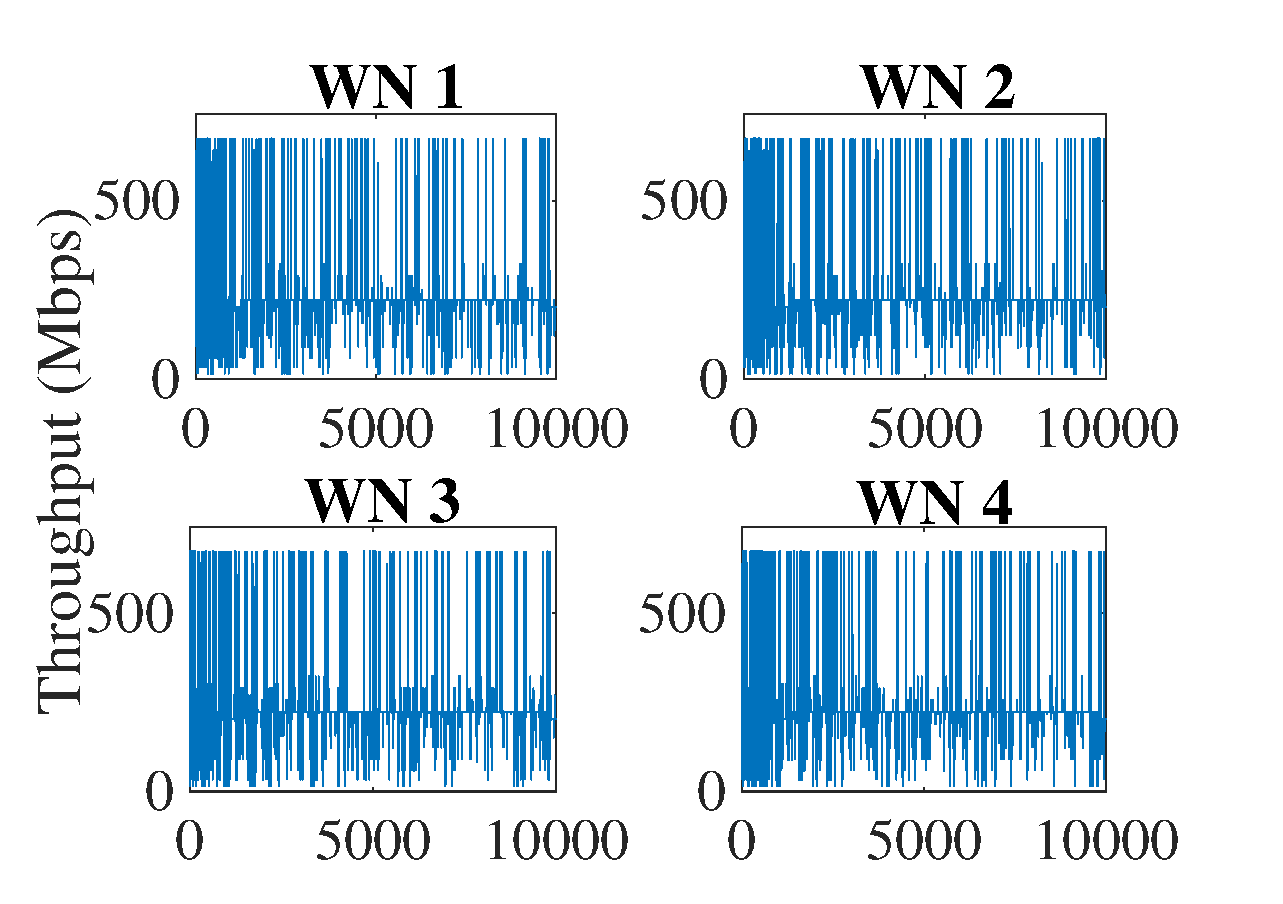
\includegraphics[width=\textwidth]{images/e_1_a1_g095_ind_tpt}
			\caption{$\varepsilon_0=1, \alpha=1, \gamma=0.95$}
			\label{fig:e_1_a1_g095_ind_tpt}
		\end{subfigure}
		\begin{subfigure}[b]{0.225\textwidth}
			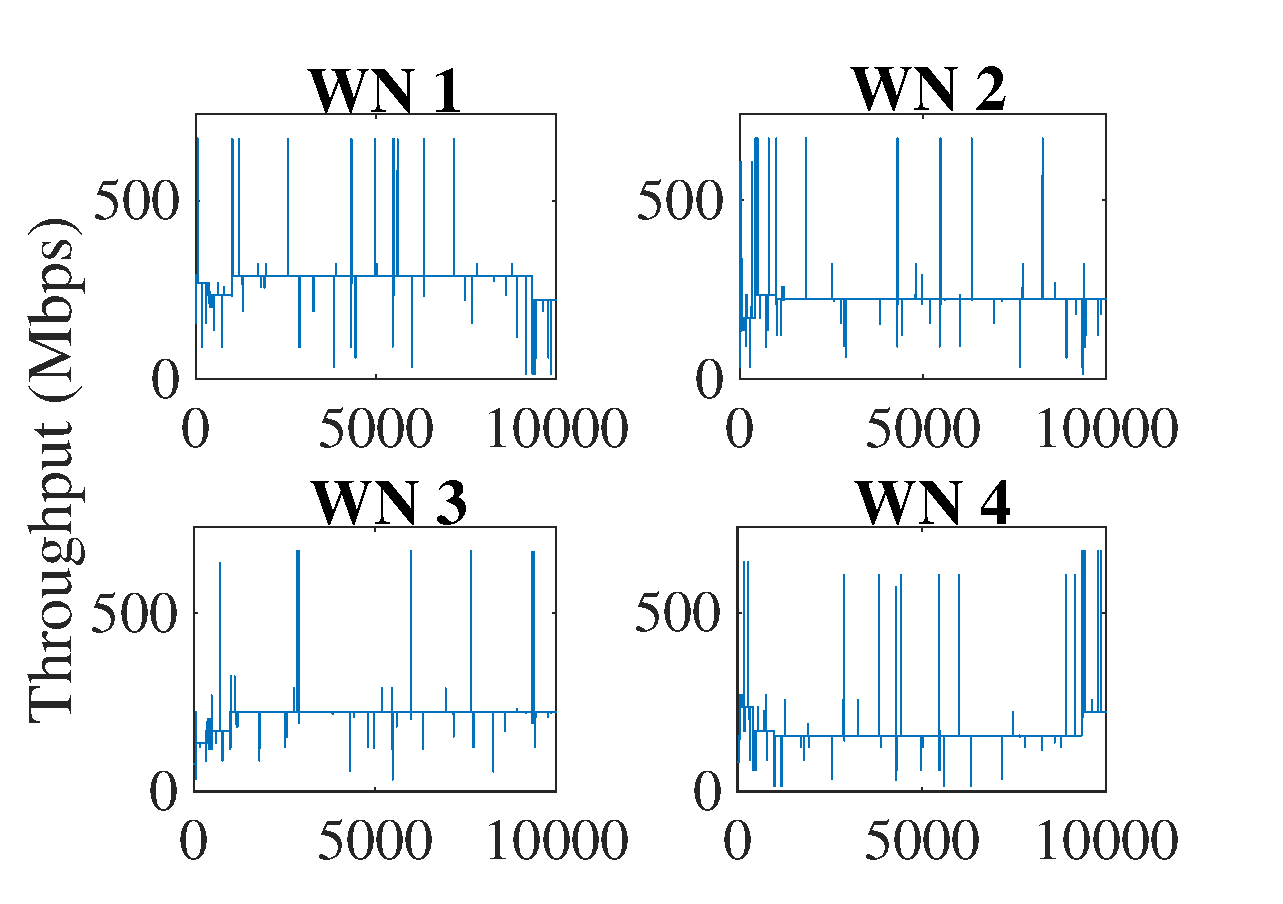
\includegraphics[width=\textwidth]{images/e_01_a_1_g_095_ind_tpt}
			\caption{$\varepsilon_0=0.1, \alpha=1, \gamma=0.95$}
			\label{fig:e_1_a_1_g_095_ind_tpt}
		\end{subfigure}
		\begin{subfigure}[b]{0.225\textwidth}
			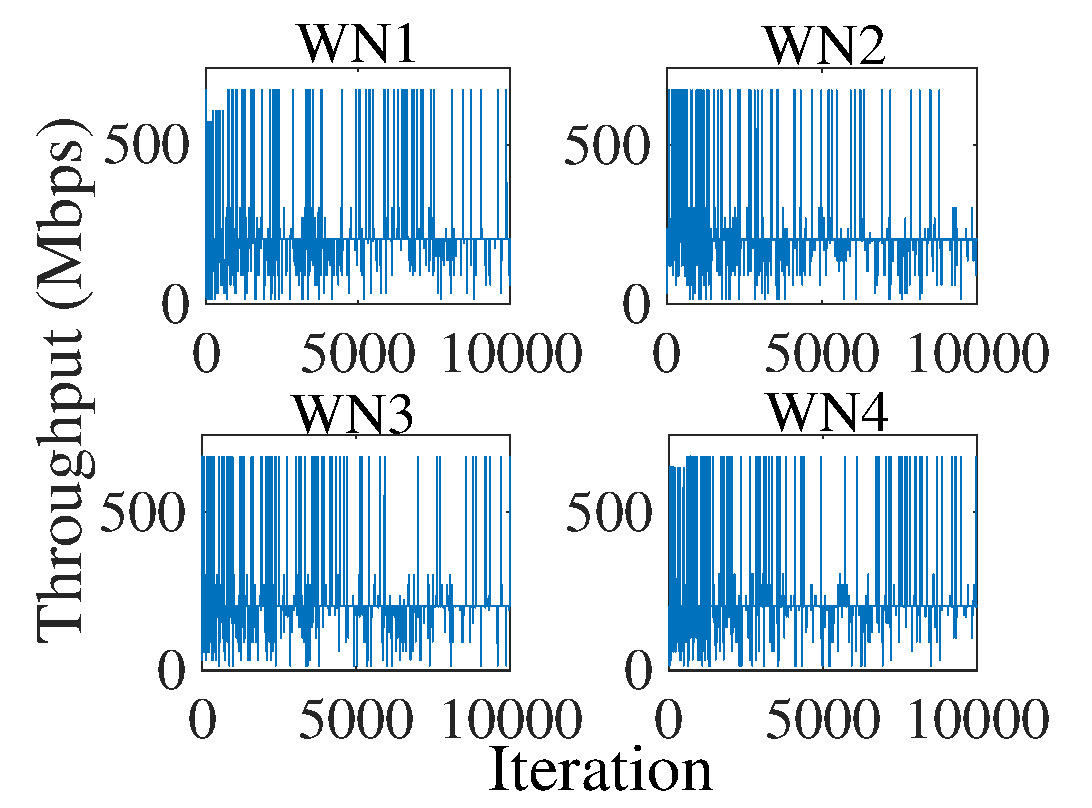
\includegraphics[width=\textwidth]{images/e_1_a_01_g_005_ind_tpt}
			\caption{$\varepsilon_0=1, \alpha=0.1, \gamma=0.05$}
			\label{fig:e_1_a_01_g_005_ind_tpt}
		\end{subfigure}
		\begin{subfigure}[b]{0.225\textwidth}
			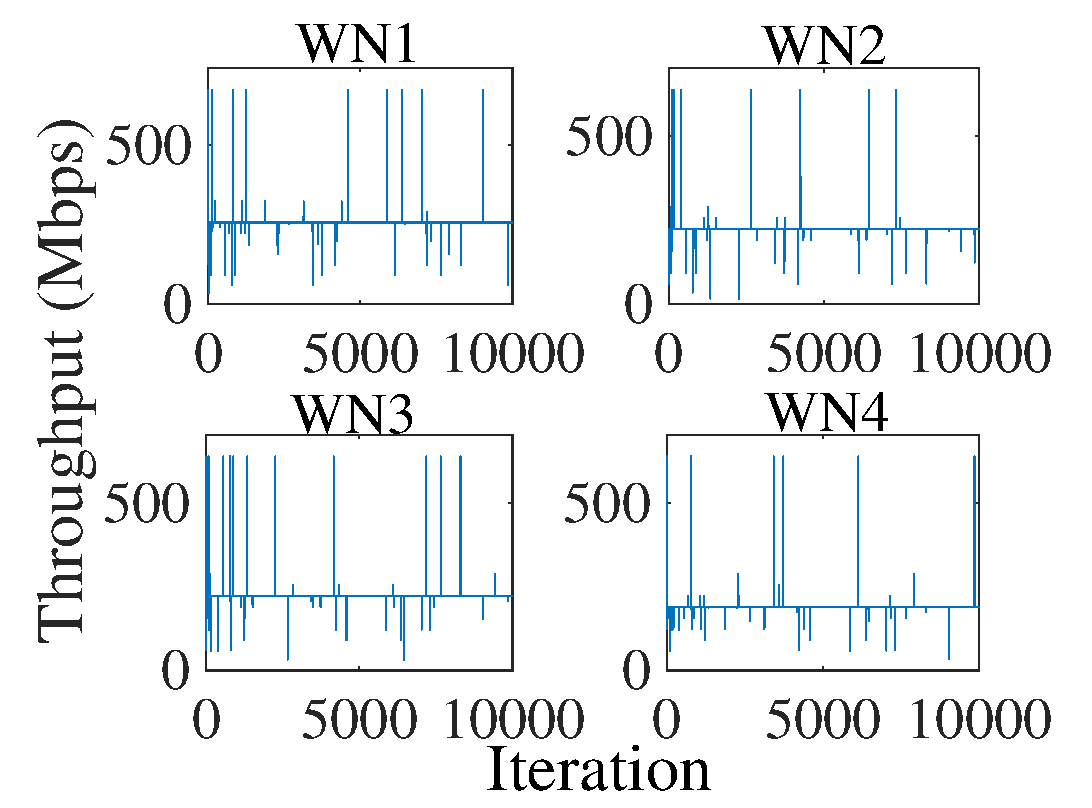
\includegraphics[width=\textwidth]{images/e_01_a_01_g_005_ind_tpt}
			\caption{$\varepsilon_0=0.1, \alpha=0.1, \gamma=0.05$}
			\label{fig:e_01_a_01_g_005_ind_tpt}
		\end{subfigure}
		\caption{Individual throughput experienced by each WN during a single (10000 iterations) simulation run for different $\varepsilon_0$, $\alpha$ and $\gamma$.}
		\label{fig:ql_params_eval_individual_tpt}
	\end{figure}
	
	%%% AVERAGE THROUGHPUT FOR EACH PARAMETER
	\begin{figure}[h!]
		\centering
		\begin{subfigure}[b]{0.225\textwidth}
			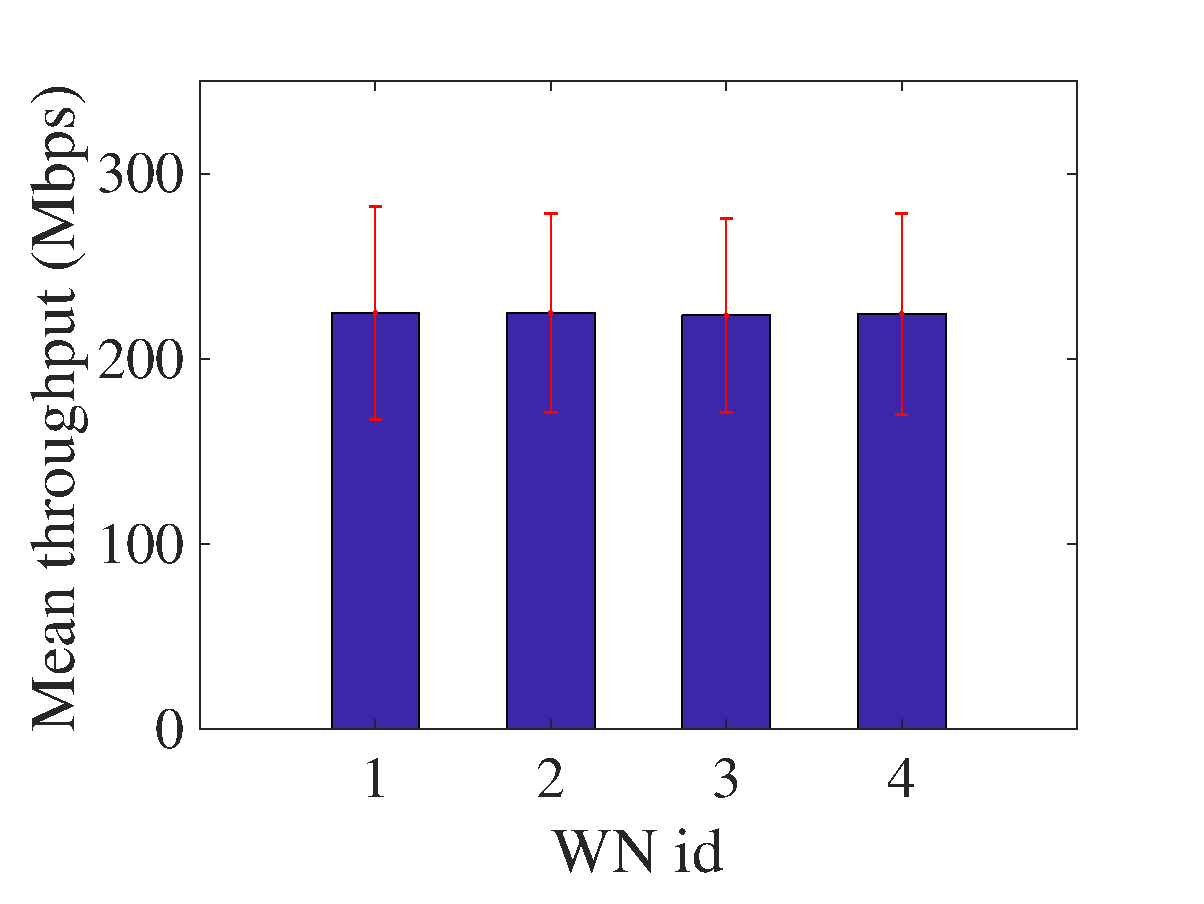
\includegraphics[width=\textwidth]{images/e_1_a1_g095_avg_tpt}
			\caption{$\varepsilon_0=1, \alpha=1, \gamma=0.95$}
			\label{fig:e1_a_1_g_0.95_avg_tpt}
		\end{subfigure}
		\begin{subfigure}[b]{0.225\textwidth}
			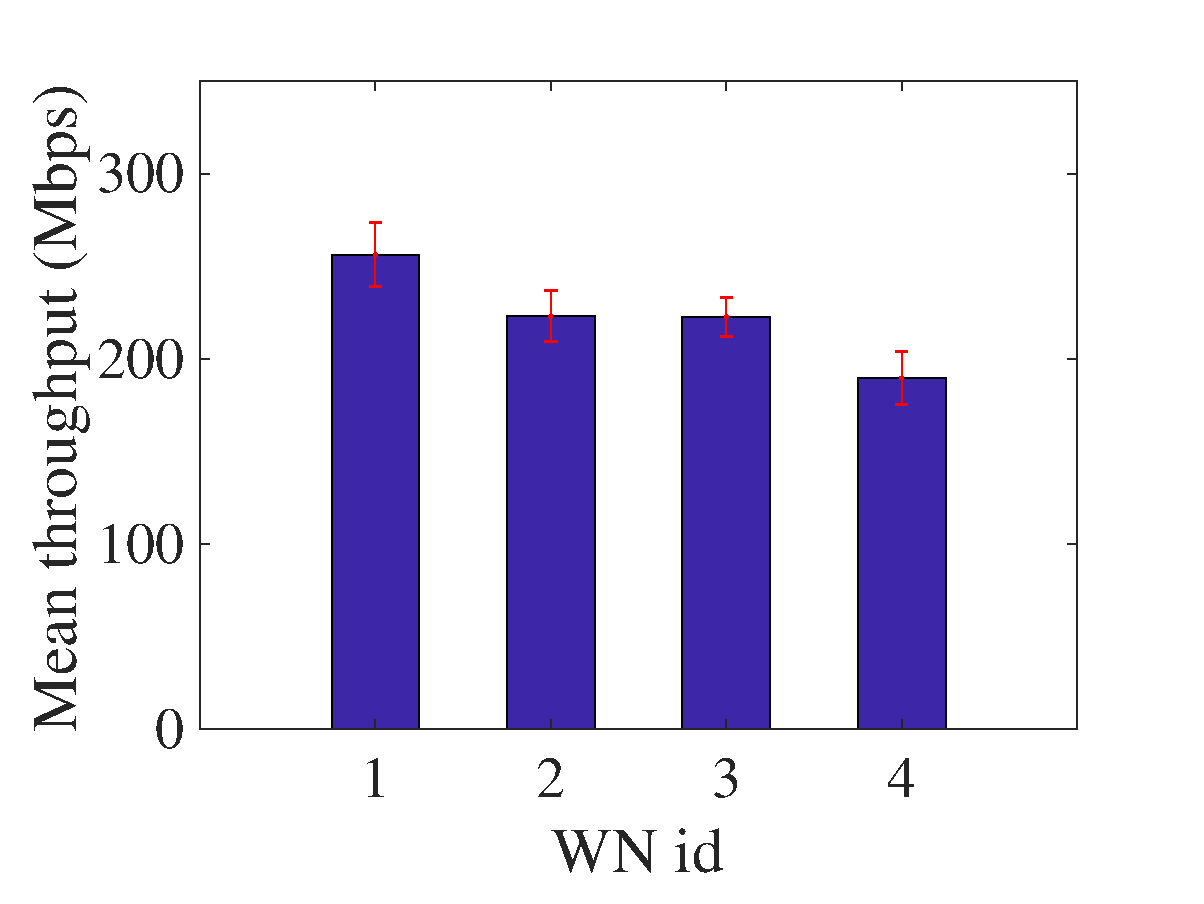
\includegraphics[width=\textwidth]{images/e_01_a_1_g_095_avg_tpt}
			\caption{$\varepsilon_0=0.1, \alpha=1, \gamma=0.95$}
			\label{fig:e_1_a_1_g_0.95_avg_tpt}
		\end{subfigure}
		\begin{subfigure}[b]{0.225\textwidth}
			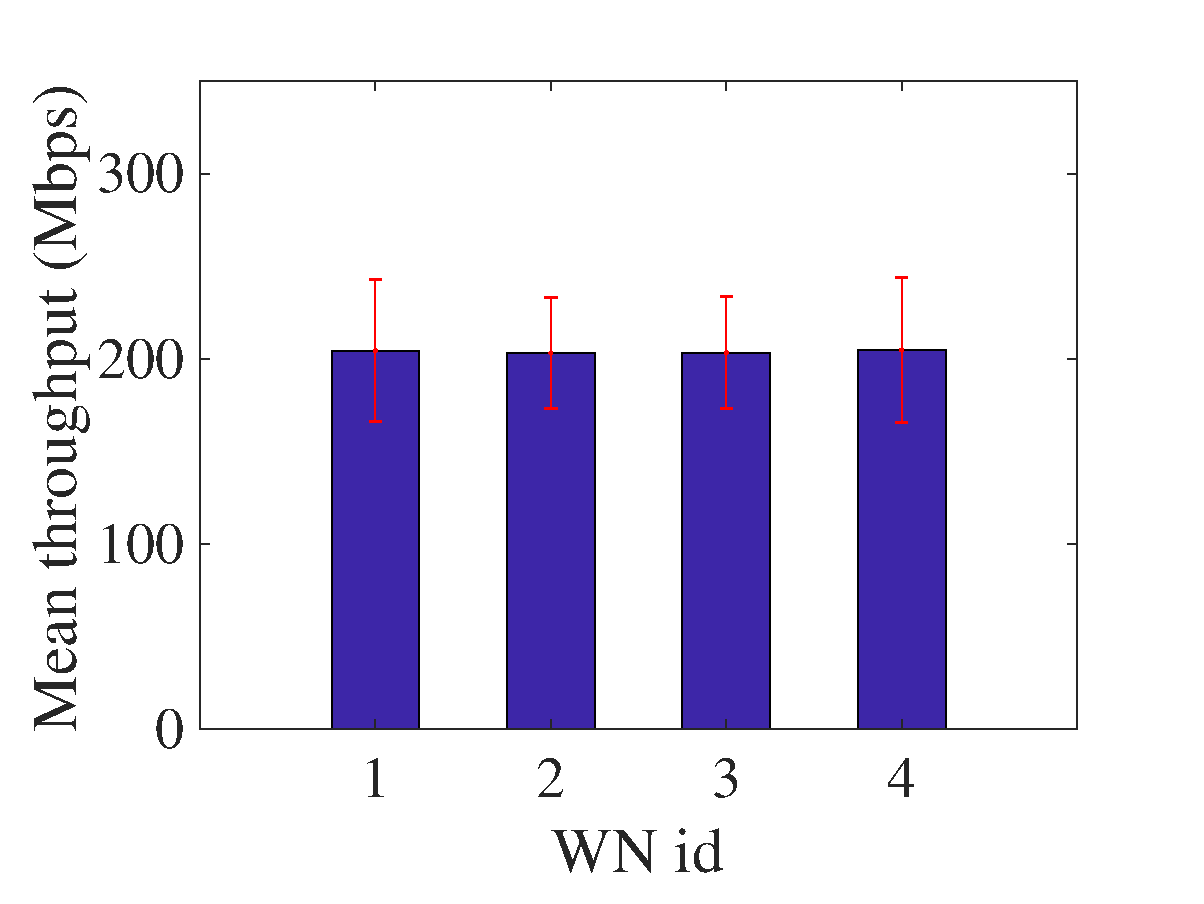
\includegraphics[width=\textwidth]{images/e_1_a_01_g_005_avg_tpt}
			\caption{$\varepsilon_0=1, \alpha=0.1, \gamma=0.05$}
			\label{fig:e_1_a_0.1_g_0.05_avg_tpt}
		\end{subfigure}
		\begin{subfigure}[b]{0.225\textwidth}
			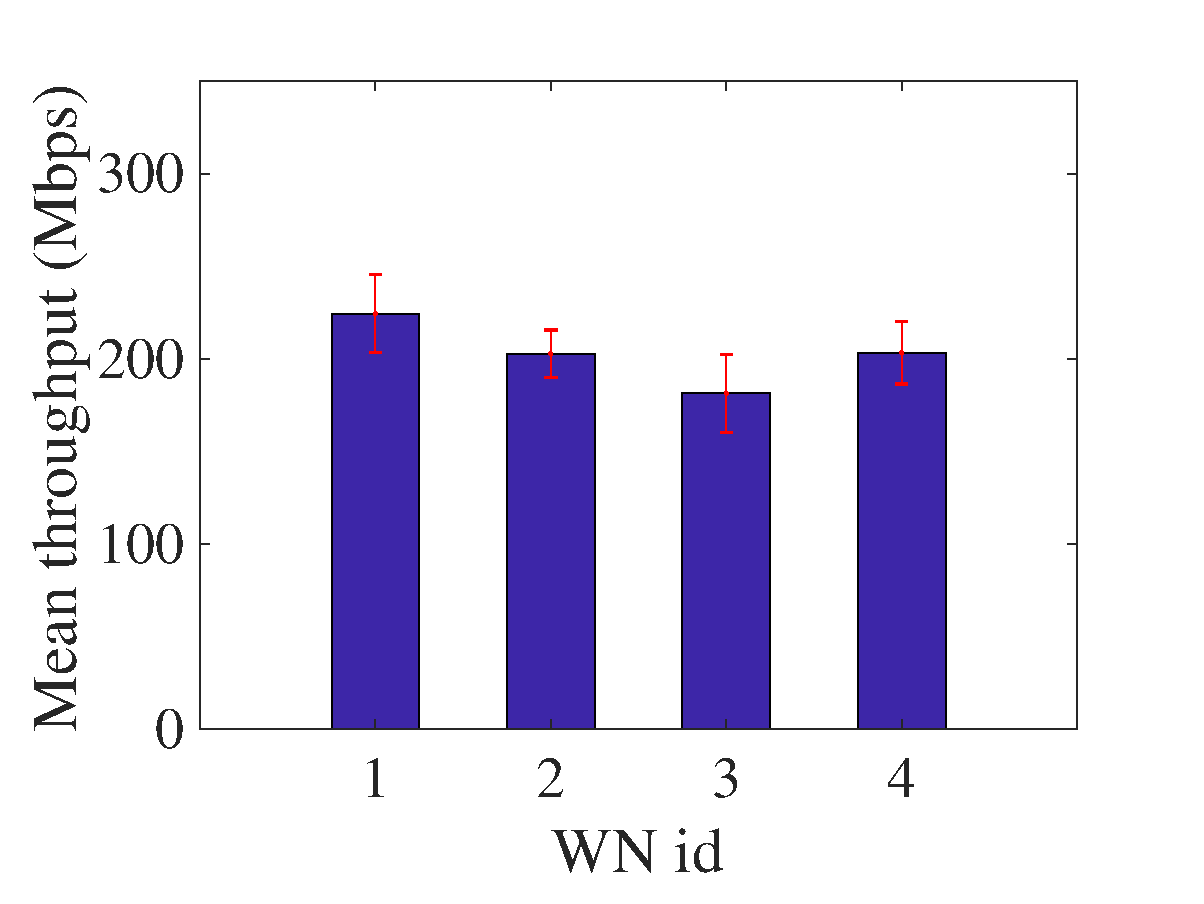
\includegraphics[width=\textwidth]{images/e_01_a_01_g_005_avg_tpt}
			\caption{$\varepsilon_0=0.1, \alpha=0.1, \gamma=0.05$}
			\label{fig:e_0.1_a_0.1_g_0.05_avg_tpt}
		\end{subfigure}
		\caption{Average throughput experienced by each WN during the last 5000 iterations of a total of 10000 iterations (in a single simulation run) and for different $\varepsilon_0$, $\alpha$ and $\gamma$.}
		\label{fig:ql_params_eval_average_tpt}
	\end{figure}
	
	%%% ACTIONS PROBABILITY FOR EACH PARAMETER	
	\begin{figure}[h!]
		\centering
		\begin{subfigure}[b]{0.225\textwidth}
			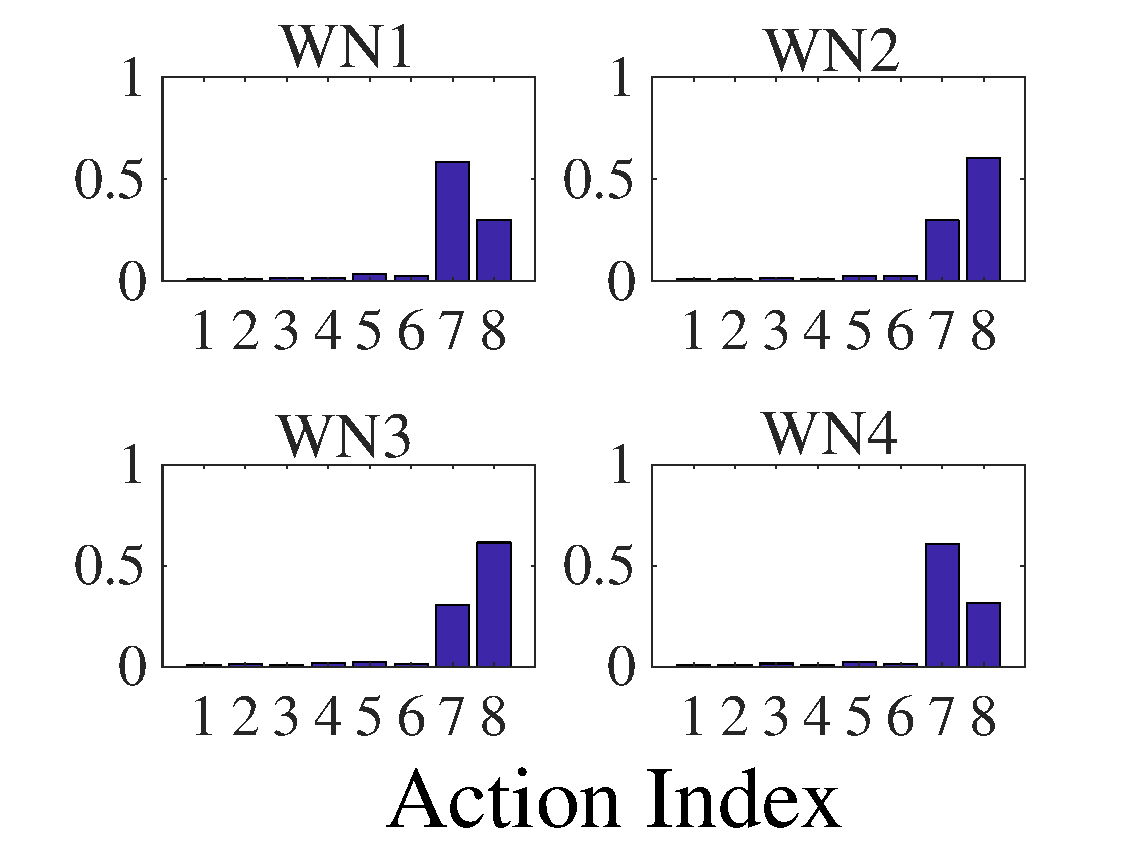
\includegraphics[width=\textwidth]{images/e_1_a1_g095}
			\caption{$\varepsilon_0=1, \alpha=1, \gamma=0.95$}
			\label{fig:e_1_a1_g095}
		\end{subfigure}
		\begin{subfigure}[b]{0.225\textwidth}
			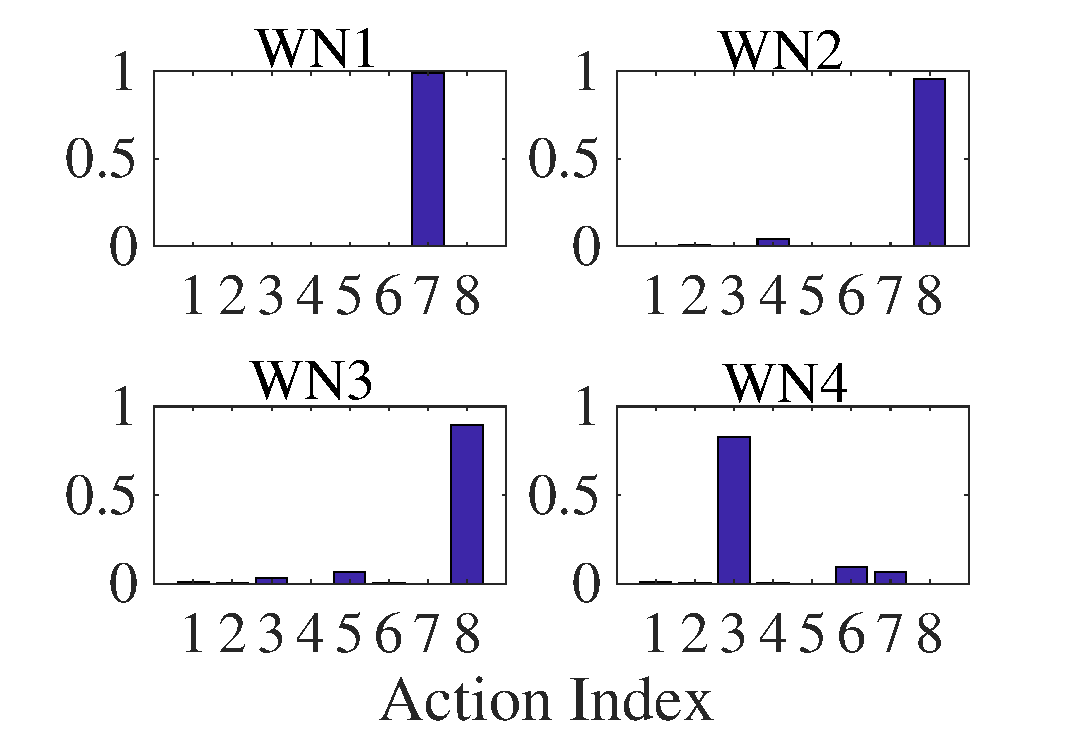
\includegraphics[width=\textwidth]{images/e_01_a_1_g_095}
			\caption{$\varepsilon_0=0.1, \alpha=1, \gamma=0.95$}
			\label{fig:e_1_a_1_g_095}
		\end{subfigure}
		\begin{subfigure}[b]{0.225\textwidth}
			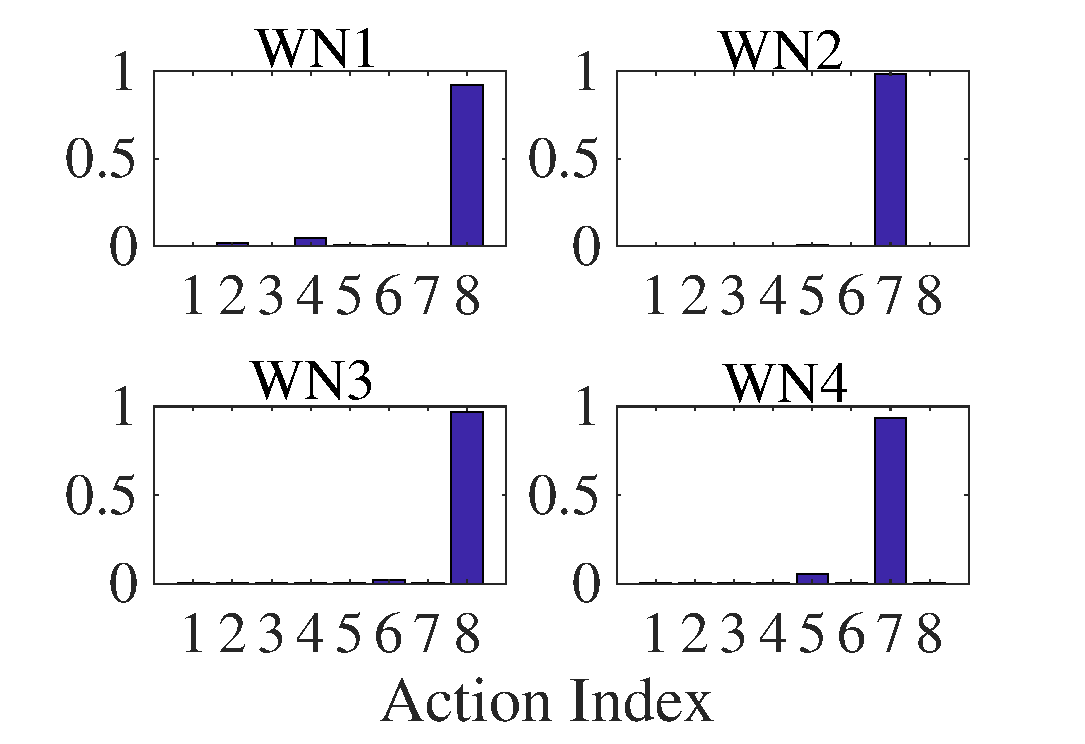
\includegraphics[width=\textwidth]{images/e_1_a_01_g_005}
			\caption{$\varepsilon_0=1, \alpha=0.1, \gamma=0.05$}
			\label{fig:e_1_a_01_g_005}
		\end{subfigure}
		\begin{subfigure}[b]{0.225\textwidth}
			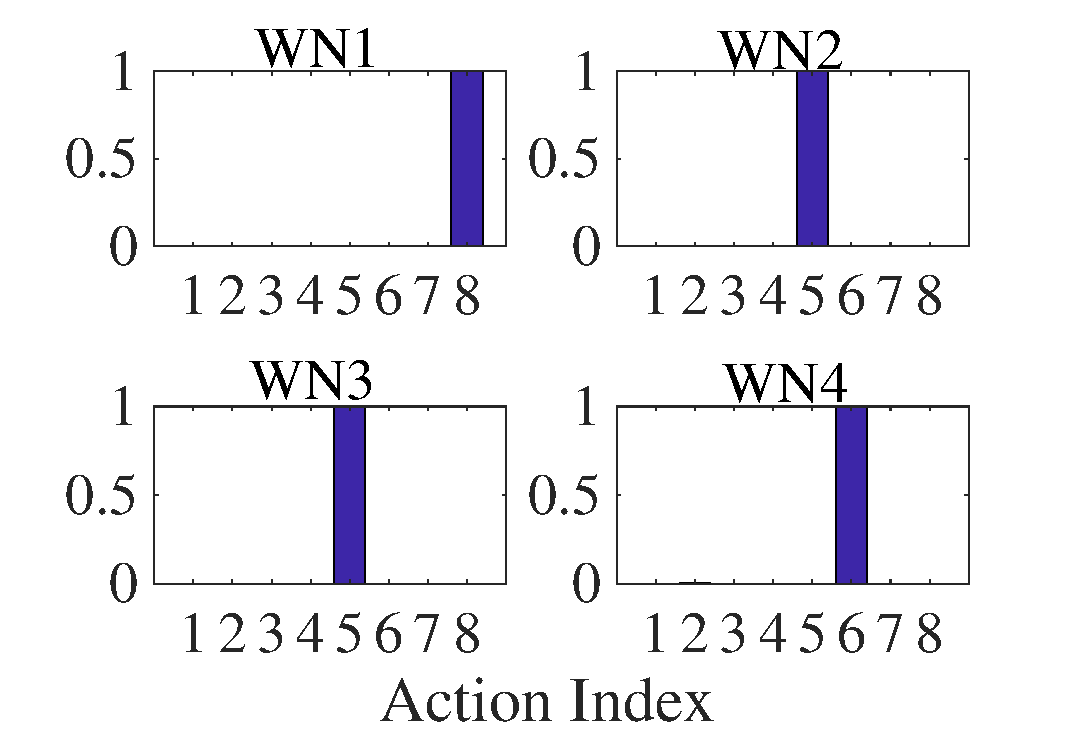
\includegraphics[width=\textwidth]{images/e_01_a_01_g_005}
			\caption{$\varepsilon_0=0.1, \alpha=0.1, \gamma=0.05$}
			\label{fig:e_01_a_01_g_005}
		\end{subfigure}
		\caption{Probability of choosing the different actions at each WN for a single (10000 iterations) simulation run and different $\varepsilon_0$, $\alpha$ and $\gamma$ values}
		\label{fig:ql_params_eval_actions_prob}
	\end{figure}
	
	%%%%%%%%%%%%%%%%%%%%%%%%%
	%%%  V. CONCLUSIONS  %%%
	%%%%%%%%%%%%%%%%%%%%%%%%%
	\section{Conclusions }
	\label{section:conclusions}		
	Decentralized Q-learning can be used to improve spatial reuse in dense wireless networks, enhancing performance as a result of exploiting the most rewarding actions. We have shown in this article, by means of a toy scenario, that Stateless Q-learning in particular allows finding good-performing configurations that achieve close-to-optimal (in terms of throughput maximization and proportional fairness) solutions. However, the competitiveness of the presented fully-decentralized environment involves the non-existence of a Nash Equilibrium. 
	Thus, we have also identified high variability in the experienced individual throughput due to the constant changes of the played actions, motivated by the fact that the reward generated by each action changes according to the opponents' ones. We have evaluated the impact of the parameters intrinsic to the learning algorithm on this variability showing that it can be reduced by a decrease of the exploration degree and learning rate. This reduction on individual throughput variability occurs at the expense of aggregate performance.
	This variability can potentially result in negative effects in the overall WN's performance. The effects of such a fluctuation in higher layers of the protocol stack can have severe consequences depending on the time scale at which they occur. For example, high throughput fluctuations may trigger congestion recovery procedures in TCP (Transmission Control Protocol). 
		
	%%%%%%%%%%%%%%%%%%%%%%%%%
	%%%  ACKNOWLEDGEMENT  %%%
	%%%%%%%%%%%%%%%%%%%%%%%%%
	\section*{Acknowledgment}
	This work has been partially supported by the Spanish Ministry of Economy and Competitiveness under the Maria de Maeztu Units of Excellence Programme (MDM-2015-0502), and by the European Regional Development Fund under grant TEC2015-71303-R (MINECO/FEDER). 
	
	%%%%%%%%%%%%%%%%%%%%%%%%%
	%%%  BIBLIOGRAPHY     %%%
	%%%%%%%%%%%%%%%%%%%%%%%%%
	\begin{thebibliography}{20}
		
		\bibitem{nie1999qlearning} Nie, J., \& Haykin, S. (1999). A Q-learning-based dynamic channel assignment technique for mobile communication systems. IEEE Transactions on Vehicular Technology, 48(5), 1676-1687.
		
		\bibitem{maghsudi2015joint} Maghsudi, S., \& Stańczak, S. (2015). Joint channel selection and power control in infrastructureless wireless networks: A multiplayer multiarmed bandit framework. IEEE Transactions on Vehicular Technology, 64(10), 4565-4578.
		
		\bibitem{akella2007self} Akella, Aditya, et al. "Self-management in chaotic wireless deployments." Wireless Networks 13.6 (2007): 737-755.
		
		\bibitem{riihijarvi2005frequency} Riihijarvi, J., Petrova, M., \& Mahonen, P. (2005, January). Frequency allocation for WLANs using graph colouring techniques. In Wireless On-demand Network Systems and Services, 2005. WONS 2005. Second Annual Conference on (pp. 216-222). IEEE.
		
		\bibitem{mhatre2007interference} Mhatre, V. P., Papagiannaki, K., \& Baccelli, F. (2007, May). Interference mitigation through power control in high density 802.11 WLANs. In INFOCOM 2007. 26th IEEE International Conference on Computer Communications. IEEE (pp. 535-543). IEEE.
		
		\bibitem{bennis2010q} Bennis, M., \& Niyato, D. (2010, December). A Q-learning based approach to interference avoidance in self-organized femtocell networks. In GLOBECOM Workshops (GC Wkshps), 2010 IEEE (pp. 706-710). IEEE.
		
		\bibitem{sutton1998reinforcement} Sutton, R. S., \& Barto, A. G. (1998). Reinforcement learning: An introduction (Vol. 1, No. 1). Cambridge: MIT press.
		
		\bibitem{watkins1992q} Watkins, C. J., \& Dayan, P. (1992). Q-learning. Machine learning, 8 (3-4), 279-292.
		
		\bibitem{jain1999throughput} Jain, R., Durresi, A., \& Babic, G. (1999). Throughput fairness index: An explanation (pp. 99-0045). Tech. rep., Department of CIS, The Ohio State University.
		
		\bibitem{bellalta2016ax} Bellalta, Boris. "IEEE 802.11 ax: High-efficiency WLANs." IEEE Wireless Communications 23.1 (2016): 38-46.  
		
	\end{thebibliography}	
	
\end{document}